%; whizzy chapter -dvi
% -initex iniptex -latex platex -format platex -bibtex jbibtex -fmt fmt
% 以上 whizzytex を使用する場合の設定。
 
%     Tokyo Debian Meeting resources
%     Copyright (C) 2012 Junichi Uekawa
%     Copyright (C) 2011, 2015 Nobuhiro Iwamatsu

%     This program is free software; you can redistribute it and/or modify
%     it under the terms of the GNU General Public License as published by
%     the Free Software Foundation; either version 2 of the License, or
%     (at your option) any later version.

%     This program is distributed in the hope that it will be useful,
%     but WITHOUT ANY WARRANTY; without even the implied warranty of
%     MERCHANTABILITY or FITNESS FOR A PARTICULAR PURPOSE.  See the
%     GNU General Public License for more details.

%     You should have received a copy of the GNU General Public License
%     along with this program; if not, write to the Free Software
%     Foundation, Inc., 51 Franklin St, Fifth Floor, Boston, MA  02110-1301 USA

%  preview (shell-command (concat "evince " (replace-regexp-in-string "tex$" "pdf"(buffer-file-name)) "&"))

%%ここからヘッダ開始。

\documentclass[mingoth,a4paper]{jsarticle}
\usepackage{monthlyreport}
% 日付を定義する、毎月変わります。
\newcommand{\debmtgyear}{2015}
\newcommand{\debmtgmonth}{4}
\newcommand{\debmtgdate}{18}
% started from zero:
% (let ((year 2013) (month 7)) (+ (* (- year 2005) 12) month -1))
\newcommand{\debmtgnumber}{125}

\begin{document}

\begin{titlepage}
\thispagestyle{empty}
% タイトルページ:編集必要な部分は最初のマクロに飛ばすこと

\vspace*{-2cm}
第\debmtgnumber{}回 東京エリア Debian 勉強会資料\\
\hspace*{-2cm}

\includegraphics{image2012-natsu/dotdeb.pdf}\\
\hfill{}\debmtgyear{}年\debmtgmonth{}月\debmtgdate{}日

% ここはアップデートすること
% 全角文字にしないとフォントのサイズが合わないので注意
\rotatebox{10}{\fontsize{30}{30} {\gt 特集:.debからPythonパッケージへの変遷}}\\

\vspace*{-2cm}
\hfill{}
\includegraphics[height=6cm]{image200502/openlogo-nd.eps}
\end{titlepage}

\newpage

\begin{minipage}[b]{0.2\hsize}
 \definecolor{titleback}{gray}{0.9}
 \colorbox{titleback}{\rotatebox{90}{\fontsize{80}{80} {\gt デビアン勉強会} }}
\end{minipage}
\begin{minipage}[b]{0.8\hsize}
\hrule
\vspace{2mm}
\hrule
\begin{multicols}{2}
\tableofcontents
\end{multicols}
\vspace{2mm}
\hrule
\end{minipage}

\dancersection{事前課題}{野島 貴英}

今回の事前課題は以下です:
\begin{enumerate}
\item 本日、何の作業をやるかを宣言ください。
\item (オプション) どこで今回の勉強会の開催を知りましたか?
\item (オプション) 何について聞きたい/参加者と話をしたいですか?
\end{enumerate}
この課題に対して提出いただいた内容は以下です。
\begin{multicols}{2}
{\small
\begin{prework}{ 野島 }
  \begin{enumerate}
  \item Q.hack timeに何をしますか?\\
    A. DDTSSなどなど\\
    http://ddtp.debian.net/ddtss/index.cgi/ja
  \item (オプション)Q.何について聞きたい/参加者と話をしたいですか?\\
    A. "Designed for Windows 10"で無理やり導入されるかもしれないSecure bootなPCについての傾向と対策とソフトウェア自由の確保の為の戦い。
  \end{enumerate}
\end{prework}

\begin{prework}{ まえだこうへい }
  \begin{enumerate}
  \item Q.hack timeに何をしますか?\\
    A. いくつか溜まっているパッケージのメンテナンス
  \item (オプション)Q.どこで今回の勉強会の開催を知りましたか?\\
    A. Debian JPのメーリングリスト
  \end{enumerate}
\end{prework}

\begin{prework}{ wskoka }
  \begin{enumerate}
  \item Q.hack timeに何をしますか?\\
    A. Tile-GX8036搭載機にdebianを移植しようと試みる
  \item (オプション)Q.どこで今回の勉強会の開催を知りましたか?\\
    A. その他
  \item (オプション)Q.何について聞きたい/参加者と話をしたいですか?\\
    A. 新しいアーキテクチャのdebian化についてご意見を伺いたい
  \end{enumerate}
\end{prework}

\begin{prework}{ keikurata }
  \begin{enumerate}
  \item Q.hack timeに何をしますか?\\
    A. 初心者なので見るだけでお願いします。
  \item (オプション)Q.どこで今回の勉強会の開催を知りましたか?\\
    A. その他
  \end{enumerate}
\end{prework}

\begin{prework}{ NOKUBI Takatsugu }
  \begin{enumerate}
  \item Q.hack timeに何をしますか?\\
    A. SimStringのパッケージ化、KAKASI関連
  \item (オプション)Q.どこで今回の勉強会の開催を知りましたか?\\
    A. その他のメーリングリスト
  \item (オプション)Q.何について聞きたい/参加者と話をしたいですか?\\
    A. mecab-ipadic-neologdのパッケージ化について
  \end{enumerate}
\end{prework}

\begin{prework}{ koedoyoshida }
  \begin{enumerate}
  \item Q.hack timeに何をしますか?\\
    A. DDTSSまたはPyconJP関連
  \item (オプション)Q.どこで今回の勉強会の開催を知りましたか?\\
    A. Debian JPのメーリングリスト
  \end{enumerate}
\end{prework}

\begin{prework}{ wbcchsyn }
  \begin{enumerate}
  \item Q.hack timeに何をしますか?\\
    A. 何かDebianに寄与する事。多分、翻訳かバグフィックス
  \item (オプション)Q.どこで今回の勉強会の開催を知りましたか?\\
    A. 友達や知り合いから直接
  \end{enumerate}
\end{prework}

\begin{prework}{ alohaug }
  \begin{enumerate}
  \item Q.hack timeに何をしますか?\\
    A. Gnuk 1.1.4がgpg4win/Win7で認識されないバグを追いかけます。
  \item (オプション)Q.どこで今回の勉強会の開催を知りましたか?\\
    A. Debian JPのメーリングリスト
  \end{enumerate}
\end{prework}

\begin{prework}{ henrich }
  \begin{enumerate}
  \item Q.hack timeに何をしますか?\\
    A. リリースノート訳
  \item (オプション)Q.どこで今回の勉強会の開催を知りましたか?\\
    A. Twitter(@tokyodebian)
  \item (オプション)Q.何について聞きたい/参加者と話をしたいですか?\\
    A. Jessieに対する不安
  \end{enumerate}
\end{prework}

\begin{prework}{ dictoss }
  \begin{enumerate}
  \item Q.hack timeに何をしますか?\\
    A. debian packageにおけるkernelの作法を調べる
  \item (オプション)Q.どこで今回の勉強会の開催を知りましたか?\\
    A. Debian JPのメーリングリスト
  \end{enumerate}
\end{prework}

\begin{prework}{ yy\_y\_ja\_jp }
  \begin{enumerate}
  \item Q.hack timeに何をしますか?\\
    A. DDTSS 
  \item (オプション)Q.どこで今回の勉強会の開催を知りましたか?\\
    A. その他
  \item (オプション)Q.何について聞きたい/参加者と話をしたいですか?\\
    A. DDTSSのレビューのお願い
  \end{enumerate}
\end{prework}

\begin{prework}{ Roger Shimizu }
  \begin{enumerate}
  \item Q.hack timeに何をしますか?\\
    A. jessieに関する検証・作業
  \item (オプション)Q.どこで今回の勉強会の開催を知りましたか?\\
    A. Twitter(@tokyodebian)
  \end{enumerate}
\end{prework}

}
\end{multicols}

\dancersection{Debian Trivia Quiz}{野島 貴英}

 Debianの昨今の話題についてのQuizです。

今回の出題範囲は\url{debian-devel-announce@lists.debian.org} や \url{debian-news@lists.debian.org}に投稿された
内容などからです。

\begin{multicols}{2}
%; whizzy-master ../debianmeetingresume201311.tex
% 以上の設定をしているため、このファイルで M-x whizzytex すると、whizzytexが利用できます。
%

\santaku
{2015/2/17にて、DPLのLucas Nussbaumにより立て直しの協力募集が行われたチームは?}
{DSA team}
{partners team}
{東京エリアDebian勉強会team}
{B}
{Debian Projectには、Debian パートナーズプログラム(https://www.debian.org/partners/)という制度があります。こちらを統括しているチームとしてpartners teamがあるのですが、昨今、こちらの構成員の時間が取れない状態らしく、対応が滞っているという状況のようです。なお、DSAはThe Debian System Administratorsというチームのことでバリバリ活動されてます。東京エリアDebian勉強会teamは当勉強会幹事の頭の中の妄想上のチームですが、頑張ってるぜ!}

\santaku
{2015/2/23に、Debianがクレジットに載せられた映画があることがindenti.caのzakの投稿で判りました。何と言う名前の映画?}
{ミレニアム ドラゴン・タトゥーの女}
{Toy Story}
{Citizenfour}
{C}
{Citizenfourというエドワード・スノーデンを題材にしたドキュメンタリー映画のクレジットのSpecial ThanksとしてDebianが入りました。imdbにもcompanyとして登録されました。Citizenfourは2015年アカデミー賞のうち長編ドキュメンタリー賞を受賞しました(http://www.imdb.com/company/co0504449/, http://www.huffingtonpost.jp/tatsuhei-morozumi/citizenfour\_b\_6741756.html)ギャガ株式会社配給で将来日本でも公開されるとのことですので、将来クレジットを確認すると良いかもしれません}

\santaku
{2015/3/31にJessieのリリース目標の日がアナウンスされました。いつでしょう?}
{4/1}
{4/18}
{4/25}
{C}
{遂に4/25がJessieのリリース目標の日取りとなりました。ただ、最悪のケースとして、Jessieにリリースに支障があるような非常に重大な問題が見つかり修正が間に合わない場合は、ずれる可能性があるとは記載されています。現在uddを参照すると、キーパッケージだけでも47個ぐらいRCバグが残ったままのようですので、Fix! Fix! なお、4/25に東京でリリースパーティーが企画されています。詳細はconnpassのDebian JPグループを見て下さいませ。}

\santaku
{2015/4/16のlucas最後のbit from DPLが流れました。こちらに記載されていたDebianからパッケージをリリースできるようにするための法的対策を検討中のソフトウェアは以下のどれ?}
{libdvdcss}
{OTR software}
{Unreal Engine4}
{A}
{なんと、libdvdcssと、ZFSが検討中らしい。もちろん、ダメになる可能性は十分にあるので、状況を静観したいと思います。libdvdcssはそのコード本体がクラッキング行為の塊なので、万一debianに入った場合、日本でdebianをミラーしても大丈夫かどうかは今後の議論ですね}

\santaku
{Debianにて開発者の属性の不均衡を正す事を目的として活動する公式チームがDebian Projectに新設したと4/16にlucasによりアナウンスがありました。なんという名前のチーム?}
{Debian Release team}
{Debian Outreach team}
{Technical Comittie}
{B}
{現在、是正すべき属性のターゲットとしては性別分布を目標としているようです。現在、Debian公式開発者の性別の割合は男性に大きく偏ってしまっています。Debianは多様性を重視するプロジェクトです。将来、性別の不均衡が是正されると良いですね。}

\santaku
{2015/4/15に選出された新DPLは誰?}
{Mehdi Dogguy}
{Gergely Nagy}
{Neil McGovern}
{C}
{Neil McGovernさんはDebian ProjectでRelease Teamで活動されるなど多数の貢献をされている方です(所信表明は:https://www.debian.org/vote/2014/platforms/neilm )。ちなみに、2015のDebian JP Project会長は岩松さんが選出されました。おめでとうございます。}







\end{multicols}

\dancersection{最近のDebian関連のミーティング報告}{野島 貴英}

\subsection{第124回東京エリアDebian勉強会}

\begin{itemize}
\item 場所はスクウェア・エニックスさんのセミナルームをお借りしての開催でした。
\item 参加者は9名でした。
\item セミナ内容は岩松さんによる「Raspberry Pi 2 Model B に Debian Jessie / armhf をインストールする」でした。
\item 残りの時間でhack timeを行い、成果発表をしました。
\item 宴会の代わりに、「祥龍房 新宿イーストサイドスクエア店」で夕食会をやりました。
\end{itemize} 

 セミナはDebian公式開発者の岩松さんにより、最近発売になったRaspberry Pi 2 Model BにDebian Jessieのarmhfアーキテクチャをインストールするお話でした。興味深い点として、Raspberry Pi 2 は、Debian Jessieのarmhfアーキテクチャがそのままで動作し、しかもDebianをインストールして、UnixBenchを取ると、Raspberry Pi (armel): Raspberry Pi 2 (armhf) = 66.5:450.8となるなど、Raspberry Piより何倍も性能が向上するようです。あわせて、cdebootstrapの詳しい動作・説明なども行われました。

 今回は参加者にて、各種 Raspberry Pi が持ち込まれ、hack timeで早速インストールなど試みる方もいらっしゃいました。DebianはいくつものCPUにもポーティングされています。組み込みでもDebianを使う人がどんどん増えると良いと思います。
 
% % (query-replace-regexp "<.*?>" "")
% % (query-replace-regexp "^[	 ]\+" "")

%-------------------------------------------------------------------------------
\dancersection{.debから Python パッケージへの変遷}{まえだこうへい}
%-------------------------------------------------------------------------------
\subsection{はじめに}

一昨年\ref{deb}、昨年\ref{debci}、現在の職場で構築および運用している Debian パッケージの自動ビルド\&ローカルアーカイブの仕組みについてお話しました(以下ローカル Debian CI と呼びます)。
昨年後半、部門での開発言語を Python \footnote{Web フレームワークには Django 及び django REST framework に統一しました。}にするという方針になり、同様の形でローカル PyPI を利用した Python パッケージ配布の仕組みを構築しました(以下 ローカル PyPI CI と呼びます)。
今まで運用して分かったメリット/デメリットや、ローカル Debian CI を必要とするケースなどについて紹介します。そして私自身が主に Python 関連の Debian パッケージをメンテナンスしていますが、これに絡めた考察を行います。

\subsection{ローカルDebian CI}

ローカル Debian CI は、git-buildpackage で管理している Git リポジトリもしくはソースパッケージを取得してビルドを行います。前者はインハウスで開発したソフトウェア、後者はバックポートする場合です。git-buildpackage / cowbuilder でのビルド、lintian でのポリシーチェック、piuparts でのインストール/アンインストールテスト、debsign\footnote{実際にはTTYなしでdebsignを実行できないため、Pythonで pydebsignを実装し、使用しています。\ref{pydebsign}}での署名、dput での reprepro へのアップロードを行います。少なくともバックポートに関してはJenkinsのプロジェクトのコピーだけで他のメンバーでも行えます。図\ref{fig:debian-ci}のような構成です。

\begin{figure}[htbp]
  \begin{center}
  \includegraphics[width=0.50\hsize]{image201504/debian-ci.eps}
  \caption{ローカルDebian CI}
  \label{fig:debian-ci}
  \end{center}
\end{figure}

\subsection{ローカル PyPI CI}

ローカル PyPI CI は同様に Jenkins を使用し、repreproに相当するローカル PyPI サーバには devpi \footnote{\url{http://doc.devpi.net/latest/} PyConJP 2014の「パッケージングの今」の資料\ref{pythonpackage}で知りました。} を使用しています。
Jenkinsのジョブスクリプトもやはり Python で実装しました。このスクリプト自体も Python パッケージ化し、ジョブ実行時にローカル PyPI からインストールして実行します。\footnote{ローカルDebian CI用のスクリプトはGitで管理し、ジョブごとにcheckoutする形式でした。}git-buildpackage/cowbuilder でのクリーンビルドに相当するクリーン環境でのテスト実行は Tox を使うことで実現しています。Tox から virtualenv 環境が作られ、Python2.7 / 3.4 でのユニットテスト\footnote{現在のOSはUbuntu Trustyのため、この2バージョンに固定。}、pylint、pychecker でのチェック、Sphinx ドキュメントのビルドのテストを行います。テストが成功するとdevpi-client \footnote{\url{https://pypi.python.org/pypi/devpi-client}、\url{http://doc.devpi.net/latest/userman/devpi_packages.html}} を使い、devpi-server にパッケージのアップロードを行います。

更に、ローカルPyPI CIにはGitHub EnterpriseからのWebhookを使ったジョブの起動と、HipChatへのテスト結果の通知の機能を実装しました。構成は図\ref{fig:pypi-ci}のようになります。

\begin{figure}[h]
  \begin{center}
  \includegraphics[width=0.6\hsize]{image201504/python-ci.eps}
  \caption{ローカルPyPI CI}
  \label{fig:pypi-ci}
  \end{center}
\end{figure}

{\scriptsize
\begin{itembox}[l]{Pythonでの開発環境の標準化}

チームメンバーのスキルレベルもまちまちであるため、品質の底上げのための次のような標準化も行いました。

\begin{itemize}
\item 開発標準化のための指針ドキュメント作成
\item Pythonパッケージのテンプレート化
\item DjangoアプリのPythonパッケージのテンプレート化
\item 独自認証システム用のモック機能付き共通ライブラリやDjangoモジュールの開発、テンプレートへの適用
\item ローカル PyPI CIをローカルの開発環境で使うためのセットアップスクリプトの提供
\item テンプレートおよびローカルPyPI CIの使い方のドキュメント作成、レクチャー
\item HipChatでの主要な変更点の案内、質疑応答
\end{itemize}

テンプレートには次のような機能を予め提供しています。

\begin{itemize}
\item Tox経由でのpytest、pytest-flake、pylint、pycheckerの実行
\item Sphinx automoduleを使ったドキュメントの自動生成、ローカルPyPIへのドキュメントアップロード
\item Djangoベストプラクティスの適用(Djangoプロジェクトのディレクトリ構成、環境ごとのsettings.pyの切替の仕組みなど)や、Djangoおよびdjango REST frameworkを含めたサンプルアプリの提供
\end{itemize}
\end{itembox}}

\subsection{before/after}

\subsubsection{パッケージ化を行えるメンバーの増加}
ローカルDebian CIの構築以前にDebianパッケージの作成のレクチャーを行ったり、ローカルDebian CIの使い方のドキュメントの作成していました。しかし、敷居が高いこともありソースパッケージの作成は他のメンバーが行える状態ではありません。

一方、Pythonパッケージはテンプレートを使い、残りのsetup.pyの必要項目さえ埋めればパッケージ化できます。これによりPythonは書けてもPythonパッケージは作ったことがないメンバーでも簡単にパッケージ化できるようになりました。

\subsubsection{開発時におけるリポジトリの利用の簡易化}
各オフィスビルからや各データセンターから\footnote{オフィスとデータセンター間は基本VPN接続ですが、一部のサービスはHTTPSでアクセスできます。これもその一つです。}でも各リポジトリはアクセスできるので、基本的にはDebianパッケージでもPythonパッケージでもその点は差がありません。しかし、パッケージ化の観点では前者は敷居が高いため、明示的にローカルの開発環境でも使う人は限られていました。\footnote{VMのインストール用のpreseedで設定しているため、知らずに使っている潜在的なユーザ及びサーバは非常に多いです。}
後者はパッケージ化が簡易であることや、アップロードもJenkinsからだけでなく、LDAPアカウントで手元からアップロード可能であり\footnote{devpi-ldap (\url{https://pypi.python.org/pypi/devpi-ldap})というモジュールを利用。}、ローカルPyPIのURLをpipの``\texttt{--index-url}''オプションで指定することで切替可能なため、利用頻度及び明示的な利用ユーザが増加しました。

\subsubsection{パッケージ化のコスト削減}

Debianパッケージでは、基本私一人で行っており独自パッケージをつくるのに掛かる労力は結構かかります。特に依存パッケージが多く、かつそれらが公式パッケージ化されていない場合には大変です。Pythonパッケージの場合には、前述の通り用意したテンプレートを使えばパッケージ化でき、アップロードも簡単であるため、比べるまでもないでしょう。

ただし、Pythonパッケージ以外ではDebianパッケージを作ることも当然あるので、この辺はパッケージを作成できるメンバーを増やす方法を検討する必要があります。\footnote{基本的には最初に公式パッケージ化にすることを検討しています。}

\subsection{ローカルDebian CIが必要なケース}
一方でDebianパッケージのカスタムビルドが必要なケースもまだあります。

\subsubsection{公式パッケージに無い}
まず、Pythonパッケージ以外で、公式パッケージにはないソフトウェアをDebianパッケージ化する場合です。これが一番多いケースです。
理想的にはライセンス上の問題がなければ、公式パッケージ化を目指したいところですが、そこは業務との兼ね合いもあり、コストがかかり過ぎる場合は割りきって、ローカルアーカイブで管理しています。ライセンス上の問題であったり、依存関係が多すぎる場合です。

\subsubsection{公式パッケージにあるがアップストリームのものを使う}

これは社内的な利用実績を重きに置く場合です。他の人が該当システムの主担当でパッケージ化を要望されるとき、アップストリームの配布するバイナリを\texttt{apt-get}でインストール可能にするためにDebianパッケージにしています。\footnote{TomcatとかOracle JDKとか。}
そうすることで外部のリポジトリを登録しなくても、ローカルアーカイブからインストールできるというメリットもあります。\footnote{Cassandraとか。}

自分が主担当の場合には公式パッケージを使うか、Sidからのバックポートを行っています。

\subsubsection{公式パッケージが古すぎて要件を満たさない場合}

この場合はバックポートの場合を行います。UbuntuのLTSやDebianのstable公式パッケージが古く、backportsに存在しないが、Sidやupstreamの配布するソースパッケージがある場合、それを使ってバックポートし、ローカルアーカイブで管理しています。

\subsubsection{Pythonパッケージでの特殊ケース}

これは現時点ではないのですが、OpenStackの導入にあたり、Ansibleで設定を行うよりも、初期のデフォルト設定を加えたカスタムビルドパッケージを使って、インストールとアップデートだけAnsibleで行った方が良いのではないか、という案です。

\subsection{Pythonパッケージの公式Debianパッケージ化について}

最後にPythonパッケージを公式Debianパッケージにすること自体について考えてみます。

\subsubsection{ユーザーの視点}
Debianパッケージとして提供されていると、\texttt{apt-get}でインストールできるのでその点が最大のメリットです。ですので、次のようなものはDebianパッケージになっていると便利です。

\begin{itemize}
\item コマンドラインツール
\item デーモン
\item 上記のパッケージに依存されているライブラリなど(直接ユーザからは見えませんが)
\end{itemize}

\subsubsection{Pythonな人の視点}

Pythonの実行環境と標準ライブラリはシステムパッケージで良いのですが\footnote{pyenvで実行環境そのものも自前で用意する、という人もいるかもしれませんが、私は違うので割愛。}、コードを書くのに使うサードパーティライブラリ自体はpipでインストールできる方が便利です。以前は、Sid上で必要なパッケージの全てをDebianパッケージ化し、Debian stableかUbuntu LTSの本番環境にもそれをバックポートしていました。が、もはや黒歴史となりました。\footnote{当時、ローカルPyPIの存在を知らなかったため、その時点で出来うる方法=Debianパッケージのローカルアーカイブを使いました。PythonパッケージのファイルをHTTPサーバーに置いて公開するというのも管理が面倒ですし。}

DebianパッケージのPythonを使う場合、virtualenv/pyvenvなどvenv環境を作るツールもDebianパッケージを使う方が、環境毎にこれらのインストールをプロジェクトのリポジトリでケアしないですみます。Toxについても下記にある通り、Debianパッケージのpython-toxを使う方が、依存するパッケージによってsetup.pyやtox.iniの記述を変更しないで済みます。


{\scriptsize
  \begin{itembox}[l]{ToxはDebianパッケージのものを使う理由}
  Toxは\texttt{python setup.py test}に統合すれば、\texttt{setup()}の\texttt{install\_requires}に指定したパッケージが\texttt{easy\_install}でローカルにダウンロードされ実行されます。

  しかし、Djangoのように\texttt{pip}しかサポートしないパッケージの場合、\texttt{setup.py test}に統合していても、まず\texttt{easy\_install}でまずローカルにインストールされるのですが、Djangoと関連のパッケージのインストールで失敗します。そのまま再度実行すると、ローカルにインストールされたファイルがあるので、\texttt{setup.py test}からの\texttt{easy\_install}はスキップされ、Toxの実行から始まります。
  ローカルで実行する場合には、これでも良いのですが、Jenkinsなどでジョブ毎にクリーン環境を作る場合、必ず失敗してしまいます。\texttt{setup.py test}に統合したToxではなく、\texttt{tox}コマンドを直接実行する場合、デフォルトでは\texttt{easy\_install}ではなく\texttt{pip}が使われ、パッケージのインストールもtoxinidirの下のtestenvのディレクトリ毎にインストールされるのでこのような問題が発生しません。
\end{itembox}
}

\subsubsection{依存するPythonパッケージに、Debianパッケージを使う場合}

依存するパッケージが既にDebianパッケージ化されている場合は、
\texttt{virtualenv}や\texttt{pyvenv}の\texttt{--system-site-packages}オプションを使えば、DebianパッケージでインストールされたPythonパッケージをvenvに使うこともできます。必要であれば、venv環境内で個別のパッケージのアップデートも可能です。

\subsubsection{開発したWebアプリをDebianパッケージにする場合}

これは公式パッケージというよりは、カスタムビルドが主なケースの話になりますが、Webアプリ自体をDebianパッケージにする場合、\texttt{start-stop-daemon}などでデーモン化し、uWSGI経由でApacheやNginxなどにリバースプロキシする設定をinitスクリプトで用意やれば、ユーザとしてはパッケージのアップデートだけで基本済むので非常に楽です。基本開発が止まっているけど、ソフトウェアそのもの需要があるなら、パッケージにすると便利です。

しかし、Webアプリとして継続的に機能追加し、リリースし続ける場合、パッケージ化するコストが高いということもありますが、一度パッケージ化してしまった後、uscan、uupdateを駆使してDebianパッケージを自動アップデート及びビルドにしたとしても、コミットからリリースまでに手順が増えるので運用に則さないと思われます。良い方法があればぜひ教えてください。\footnote{以前は、ビルド済み配布物の作成に\texttt{bdist\_deb}がありましたが、今は無くなったようです。}

\subsection{Pythonパッケージを公式Debianパッケージにすべきか}
デーモンやコマンドラインツールのパッケージ化であれば、Pythonでないユーザにとってメリットがあるので、パッケージ\&メンテナンスできるならやると良いでしょう。一方、ライブラリだけが目的なら、そもそもPythonでないユーザには使われない上、Pythonな人もpipでインストールするほうが利便性が高いので基本やる必要がないと思います。
一方、C bindingのPythonライブラリの場合、そもそもPyPIに公開されていないこともあります。そういうケースではDebianパッケージは必須になるでしょう。\footnote{例えば、netsnmp-pythonなどはDebianパッケージにしかありません。libvirt-pythonはPyPIにあります。}

Debianパッケージの作り方自体を学ぶのであれば、Pythonは比較的パッケージ化がしやすいのではないかと思います。dh-pythonパッケージに含まれる、\texttt{pybuild}コマンドのおかげで、以前よりもGolangのパッケージ化並に簡単になりました。\texttt{しかし、Golangの方が簡単です。これもあまりパッケージ化する意義が無い言語ですが…。}


ところで以前、PyPIに登録されているPythonパッケージを全部自動でDebianパッケージ化する、という話もあった気がしますが、どこ行ったのでしょうか。

\subsection{まとめ}

基本、Debianパッケージ化するのをやめたら幸せになりました。が、部分的にはDebianパッケージにすることで利便性があがるので、ケースバイケースでやると良いのではないでしょうか、というのが、私の中での結論になっています。
ぜひ、他の方のお考えもお聞かせ頂ければと思います。

そういえば、Rubyでも同じ話が既にされていたと思うのですけど、結局どうなったのでしたでしょうか?

{\scriptsize
\begin{thebibliography}{9}
\bibitem{ref:deb}``とあるWeb企業でのDebianシステムの使い方。``, \url{http://gum.debian.or.jp/2013/session/437.html}
  \label{deb}
\bibitem{ref:debci}``JenkinsでのDebianパッケージ自動化``, \url{http://tokyodebian.alioth.debian.org/2014-07.html}
  \label{debci}
\bibitem{ref:pydebsign}``I made debsign of Python libary that can be run without a TTY``, \url{http://d.palmtb.net/2014/05/28/i_made_debsign_of_python_libary_that_can_be_run_without_a_tty.html}
  \label{pydebsign}
  \bibitem{ref:oraclejdk}``Retrieve and generate debian package of Oracle JDK``, \url{http://d.palmtb.net/2014/04/16/retrieve_and_generate_debian_package_of_oracle_jdk.html}
  \bibitem{ref:debci2}``How to build custom Debian package automatically by Jenkins``, \url{http://d.palmtb.net/2014/04/12/how_to_build_custom_debian_package_automatically_by_jenkins.html}
  \bibitem{ref:tomcat7}``Issue deploying Jenkins to Tomcat7 Debian package in Wheezy``, \url{http://d.palmtb.net/2014/03/27/issue_deploying_jenkins_to_tomcat7_debian_package_in_wheezy.html}
  \bibitem{ref:pythonpackage}``パッケージングの今``, \url{http://www.slideshare.net/aodag/ss-39068785}
    \label{pythonpackage}
\end{thebibliography}
}

\newpage

\vspace*{15cm}
\hrule
\vspace{2mm}

\includegraphics[width=2cm]{image200502/openlogo-nd.eps}
\noindent \Large \bf Debian 勉強会資料\\
\noindent \normalfont \debmtgyear{}年\debmtgmonth{}月\debmtgdate{}日 \hspace{5mm}  初版第1刷発行\\
\noindent \normalfont 東京エリア Debian 勉強会 (編集・印刷・発行)\\
\hrule

\end{document}
